\documentclass[tikz]{standalone}

\usetikzlibrary{arrows, shapes, positioning}

\begin{document}
    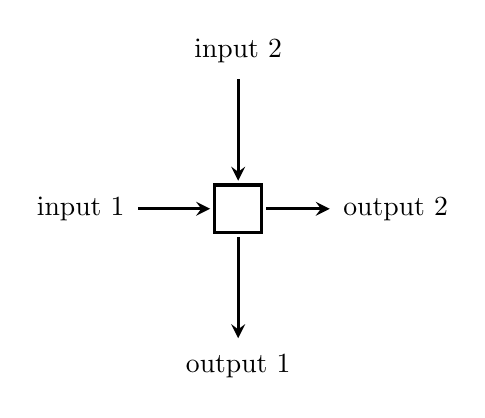
\begin{tikzpicture}[scale=4, >=stealth, node distance=2cm, shorten >=1pt, shorten <=1pt, minimum size=0.6cm, very thick]

        \node[rectangle, draw] (A) {};

        \node[left of=A] (i0) {input 1};
        \node[above of=A] (i1) {input 2};

        \node[below of=A] (o0) {output 1};
        \node[right of=A] (o1) {output 2};

        \draw[->] (i0.east) -- (A.west);
        \draw[->] (i1.south) -- (A.north);

        \draw[->] (A.south) -- (o0.north);
        \draw[->] (A.east) -- (o1.west);

    \end{tikzpicture}
\end{document}
